\documentclass[12pt]{article}
\usepackage[utf8]{inputenc}
\usepackage{tikz, url}
\usepackage[a4paper,width=150mm,top=25mm,bottom=25mm]{geometry}
\usepackage{verbatim, hyphenat}

\title{
{Updated statement of the nature and goals my honors project} \\
}

\author{Joel Savitz}

\begin{document}

\maketitle

\section{Purpose}

I began
this honors project
as a two-person endeavour,
but after careful thought and consideration,
I propose that the best way forward
for all parties involved
is for us to complete
our own aspects
of this project
individually.

Then,
given the sudden change
in the nature of the project,
and due in no small amount as well
to the vagueness of the original proposal,
this document summarizes
my individual accomplishments
and my work with another partner
on the aspects of this project
that have resulted in a progress
towards mature deliverables
and proposes specific goals
to clarify the requirements
necessary for the honors college and I
to consider this project to be completed.

\section{Project Status} 

So far, I have done the following:

\begin{enumerate}
	\item Implemented the core features of \texttt{\texttt{python3-libgpiod-rpi}} \cite{gpiolib}
	\item Wrote a detailed functional and techincal specification for \texttt{python3-libgpiod-rpi} \cite{spec}
	\item Thouroughly analyzed and documented the original \texttt{RPi.GPIO} \cite{rpi_gpio}
	\item Contributed a few minor bug fixes to the open source \texttt{libgpiod} library
		\cite{libgpiod_commit1} \cite{libgpiod_commit2}
\end{enumerate}

\section{Enumeration of Goals}

This section enumerates my remaining goals for this project.
I group goals into three categrories.
The first,
essential goals,
are items which I completely commit to.
The second,
preferred goals,
are items that I would really like to do
but that I  would accept not completing
if they became infeasible.
The third,
breakthrough goals,
are items that would be nice to complete
but are secondary to more pressing matters.


I sketch out a rough timeline
of the months
in which I aim to complete these goals
in figure \ref{timeline}.

\subsection{Essential Goals}

\begin{enumerate}

	\item[A1.]  Implementation and verification of \texttt{python3-libgpiod-rpi} 1.0 as specified
	\item[A2.] Submission of archivable document consisting of an analysis of the project as well the specification
	\item[A3.] Presentation of the project and it's outputs to the honors college

\end{enumerate}

\subsection{Preferred Goals}

\begin{enumerate}
	\item[B1.] Inclusion of \texttt{python3-libgpiod-rpi} in official Fedora package repositiories
	\item[B2.] Inclusion of \texttt{python3-libgpiod-rpi} in the Arch User Repository
\end{enumerate}

\subsection{Breakthrough Goals}

\begin{enumerate}
	\item[C1.]  Presentation of the library at some technology conference
	\item[C2.]  Acceptance of some patch to upstream mainline Linux
\end{enumerate}

\begin{figure}

  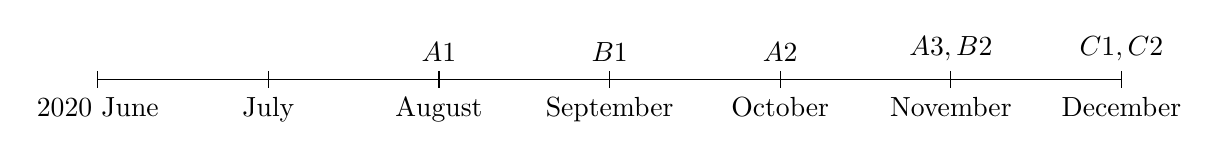
\begin{tikzpicture}
    % draw horizontal line   
    \draw (0,0) -- (13,0);

    % draw vertical lines
    \foreach \x in {0,2.166, 4.333, 6.5, 8.666, 10.833, 13}
      \draw (\x cm,3pt) -- (\x cm,-3pt);

    % draw nodes
      \draw (0,0) node[below=3pt] {$ \textrm{2020 June}$} node[above=3pt] {$  $};
      \draw (2.166,0) node[below=3pt] {$ \textrm{July} $} node[above=3pt] {$  $};
      \draw (4.333,0) node[below=3pt] {$ \textrm{August} $} node[above=3pt] {$ A1 $};
      \draw (6.500,0) node[below=3pt] {$ \textrm{September} $} node[above=3pt] {$ B1 $};
      \draw (8.666,0) node[below=3pt] {$ \textrm{October} $} node[above=3pt] {$ A2 $};
      \draw (10.833,0) node[below=3pt] {$ \textrm{November} $} node[above=3pt] {$ A3,B2 $};
    \draw (13,0) node[below=3pt] {$ \textrm{December} $} node[above=3pt] {$ C1, C2 $};
  \end{tikzpicture}

  \centering
  \caption{My new proposed timeline for this project}
  \label{timeline}

\end{figure}

\bibliographystyle{plain}
\bibliography{sources}

\end{document}
